%%%%%%%%%%%%%%%%%%%%%%%%%%%%%%%%%%%%%%%%%%%%%%%%%%%%%%%%%%%%%%%%%%%%%%%%%%%%%%%%
%%%%%%%%%%%%%%%%%%   Vorlage für eine Abschlussarbeit   %%%%%%%%%%%%%%%%%%%%%%%%
%%%%%%%%%%%%%%%%%%%%%%%%%%%%%%%%%%%%%%%%%%%%%%%%%%%%%%%%%%%%%%%%%%%%%%%%%%%%%%%%

% Erstellt von Maximilian Nöthe, <maximilian.noethe@tu-dortmund.de>
% ausgelegt für lualatex und Biblatex mit biber

% Kompilieren mit
% latexmk --lualatex --output-directory=build thesis.tex
% oder einfach mit:
% make

\documentclass[
  tucolor,       % remove for less green,
  BCOR=12mm,     % 12mm binding corrections, adjust to fit your binding
  parskip=half,  % new paragraphs start with half line vertical space
  open=any,      % chapters start on both odd and even pages
  cleardoublepage=plain,  % no header/footer on blank pages
]{tudothesis}


% Warning, if another latex run is needed
\usepackage[aux]{rerunfilecheck}

% just list chapters and sections in the toc, not subsections or smaller
\setcounter{tocdepth}{1}

%------------------------------------------------------------------------------
%------------------------------ Fonts, Unicode, Language ----------------------
%------------------------------------------------------------------------------
\usepackage{fontspec}
\defaultfontfeatures{Ligatures=TeX}  % -- becomes en-dash etc.

% load english (for abstract) and ngerman language
% the main language has to come last
\usepackage[american, ngerman]{babel}

% intelligent quotation marks, language and nesting sensitive
\usepackage[autostyle]{csquotes}

% microtypographical features, makes the text look nicer on the small scale
\usepackage{microtype}

%------------------------------------------------------------------------------
%------------------------ Math Packages and settings --------------------------
%------------------------------------------------------------------------------

\usepackage{amsmath}
\usepackage{amssymb}
\usepackage{mathtools}

% Enable Unicode-Math and follow the ISO-Standards for typesetting math
\usepackage[
  math-style=ISO,
  bold-style=ISO,
  sans-style=italic,
  nabla=upright,
  partial=upright,
  warnings-off={mathtools-colon,mathtools-overbracket}, % suppress some unnecessary warnings
]{unicode-math}
\setmathfont{Latin Modern Math}

% nice, small fracs for the text with \sfrac{}{}
\usepackage{xfrac}


%------------------------------------------------------------------------------
%---------------------------- Numbers and Units -------------------------------
%------------------------------------------------------------------------------

\usepackage[
  locale=DE,
  separate-uncertainty=true,
  per-mode=symbol-or-fraction,
]{siunitx}

%------------------------------------------------------------------------------
%-------------------------------- tables  -------------------------------------
%------------------------------------------------------------------------------

\usepackage{booktabs}       % \toprule, \midrule, \bottomrule, etc

%------------------------------------------------------------------------------
%-------------------------------- graphics -------------------------------------
%------------------------------------------------------------------------------

\usepackage{graphicx}
% currently broken
% \usepackage{grffile}

% allow figures to be placed in the running text by default:
\usepackage{scrhack}
\usepackage{float}
\floatplacement{figure}{htbp}
\floatplacement{table}{htbp}

% keep figures and tables in the section
\usepackage[section, below]{placeins}


%------------------------------------------------------------------------------
%---------------------- customize list environments ---------------------------
%------------------------------------------------------------------------------

\usepackage{enumitem}

%------------------------------------------------------------------------------
%------------------------------ Bibliographie ---------------------------------
%------------------------------------------------------------------------------

\usepackage[
  backend=biber,   % use modern biber backend
  autolang=hyphen, % load hyphenation rules for if language of bibentry is not
                   % german, has to be loaded with \setotherlanguages
                   % in the references.bib use langid={en} for english sources
]{biblatex}
\addbibresource{references.bib}  % the bib file to use
\DefineBibliographyStrings{german}{andothers = {{et\,al\adddot}}}  % replace u.a. with et al.


% Last packages, do not change order or insert new packages after these ones
\usepackage[pdfusetitle, unicode, linkbordercolor=tugreen, citebordercolor=tugreen]{hyperref}
\usepackage{bookmark}
\usepackage[shortcuts]{extdash}

%------------------------------------------------------------------------------
%-------------------------    Angaben zur Arbeit   ----------------------------
%------------------------------------------------------------------------------

\author{Maximilian Nöthe}
\title{\LaTeX-Dokumentenklasse und Vorlage für Abschlussarbeiten an der TU Dortmund}
\date{2014}
\birthplace{Castrop-Rauxel}
\chair{Lehrstuhl für Experimentelle Physik V}
\division{Fakultät Physik}
\thesisclass{Bachelor of Science}
\submissiondate{31. September 2015}
\firstcorrector{Prof.~Dr.~Erstgutachter}
\secondcorrector{Prof.~Dr.~Zweitgutachter}

% tu logo on top of the titlepage
\titlehead{
\includegraphics[height=1.5cm]{logos/tu-logo.pdf}}

\begin{document}
\frontmatter
\thispagestyle{empty}
\setcounter{page}{2}
\section*{Hinweise}
Empfohlen wird die Verwendung dieser Vorlage mit der jeweils aktuellsten TeXLive Version (Linux, Windows) bzw. MacTeX Version (MacOS).
Aktuell ist dies TeXLive 2016. Download hier:
\begin{center}
  \ttfamily\url{https://www.tug.org/texlive/}
\end{center}
Bei Verwendung von TexLive Versionen 2014 und älter sollte
die Zeile
\begin{center}
\verb+\RequirePackage{fixltx2e}+ 
\end{center}
als erste Zeile der Präambel noch vor der Dokumentenklasse eingefügt werden.
Dies lädt diverse Bugfixes für LaTeX, die ab TexLive 2015 Standard sind.

Die Vorlage \texttt{thesis.tex} ist für die Kompilierung mit \texttt{lualatex} ausgelegt, mit wenigen Anpassungen kann sie aber auch mit \texttt{pdflatex} oder \texttt{xelatex} verwendet werden. 
Die Dokumentenklasse \texttt{tudothesis.cls} kann mit allen drei Programmen verwednet werden.

Achten Sie auch auf die Kodierung der Quelldateien.
Bei Verwendung von Xe\LaTeX\ oder Lua\LaTeX\ (empfohlen) müssen die
Quelldateien UTF-8 kodiert sein.
Bei Verwendung von pdf\LaTeX\ nutzen Sie die Pakete \texttt{inputenc} und \texttt{fontenc} mit der korrekten Wahl der Kodierungen.

Eine aktuelle Version dieser Vorlage steht unter 
\begin{center}
  \ttfamily\url{https://github.com/maxnoe/tudothesis}
\end{center}
zur Verfügung.

Alle verwendeten Pakete werden im \LaTeX{} Kurs von Pep et al.\ erklärt:
\begin{center}
  \ttfamily\url{http://toolbox.pep-dortmund.org/notes}
\end{center}

Für Rückmeldungen und bei Problemen mit der Klasse oder Vorlage, bitte ein \emph{Issue} auf GitHub aufmachen oder eine Email an
\href{mailto:maximilian.noethe@tu-dortmund.de}{maximilian.noethe@tu-dortmund.de} schreiben.

Wenn Sie die Dokumentenklasse mit der Option \texttt{tucolor} laden, werden verschiedene Elemente in TU-Grün gesetzt.

\maketitle

% Gutachterseite
\makecorrectorpage

% hier beginnt der Vorspann, nummeriert in römischen Zahlen
\thispagestyle{plain}

\section*{Kurzfassung}
Hier steht eine Kurzfassung der Arbeit in deutscher Sprache inklusive der Zusammenfassung der
Ergebnisse.
Zusammen mit der englischen Zusammenfassung muss sie auf diese Seite passen.

\section*{Abstract}
\begin{foreignlanguage}{english}
The abstract is a short summary of the thesis in English, together with the German summary it has to fit on this page.
\end{foreignlanguage}

\tableofcontents

\mainmatter
% Hier beginnt der Inhalt mit Seite 1 in arabischen Ziffern
\chapter{Einleitung}
Hier folgt eine kurze Einleitung in die Thematik der Bachelorarbeit.
Die Einleitung muss kurz sein, damit die vorgegebene Gesamtlänge der 
Arbeit von 25 Seiten nicht überschritten wird. 
Die Beschränkung der Seitenzahl sollte man ernst nehmen,
da Überschreitung zu Abzügen in der Note führen kann. 
Um der Längenbeschränkung zu genügen, darf auch nicht an der Schriftgröße,
dem Zeilenabstand oder dem Satzspiegel (bedruckte Fläche der Seite) manipuliert werden.

\chapter{Struktur der Arbeit}

Eine mögliche Struktur der Arbeit sieht wie folgt aus:

\begin{enumerate}
    \item \textbf{Einleitung}\\
        In der \emph{kurzen} Einleitung wird die Motivation für die Arbeit
        dargestellt und ein Einblick in die kommenden Kapitel gegeben.
    \item \textbf{Theoretische Grundlagen}\\
        Alles was an theoretischen Grundlagen benötigt wird, sollte auch eher kurz gehalten werden.
        Statt Grundlagenwissen zu präsentieren, eher auf die entsprechenden Lehrbücher verweisen.
        Etwa: Tiefer gehende Informationen zur klassischen Mechanik entnehmen Sie bitte \cite{kuypers}.
    \item \textbf{Ergebnisse} \\
        Der eigentliche Teil der Arbeit, das was getan wurde.
    \item \textbf{Zusammenfassung und Ausblick} \\
        Zusammenfassung der Ergebnisse, Optimierungsmöglichkeiten, mögliche weitergehende Untersuchungen.
\end{enumerate}

Die Gliederung sollte auf der einen Seite nicht zu fein sein, auf der anderen Seite
sollten sich klar unterscheidende Abschnitte auch kenntlich gemacht werden.

In der hier verwendeten \KOMAScript-Klasse \texttt{scrbook} ist die oberste Gliederungsebene,
die in der Bachelorarbeit verwendet werden sollte, das \texttt{\textbackslash chapter}.

Ein Kapitel sollte erst dann in tiefere Gliederungsebenen unterteilt werden, wenn es auch wirklich etwas zu unterteilen gibt. Es sollte keine Kapitel mit nur einem Unterkapitel (\texttt{\textbackslash section}) geben.

In dieser Vorlage ist die Tiefe des Inhaltsverzeichnisses auf \texttt{chapter} und \texttt{section} beschränkt. Möchten Sie diese Beschränkung aufheben, entfernen Sie den Befehl
\begin{verbatim}
            \setcounter{tocdepth}{1}
\end{verbatim}
aus der Präambel oder ändern Sie den Zahlenwert entsprechend. Das Inhaltsverzeichnis sollte für eine Bachelorarbeit auf eine Seite passen.

\chapter{Wichtige Hinweise zum Dokument}\label{make}

Diese Vorlage ist auf die Kompilierung mit \texttt{lualatex} ausgelegt. 
Als Dokumentenklasse  wird die \KOMAScript\-Klasse \texttt{scrbook} verwendet.
Falls Sie Änderungen am Layout vornehmen möchten, lesen Sie die \KOMAScript-Dokumentation: \cite{koma}.

Eine umfangreiche Einführung in die moderne Verwendung von \LaTeX{} gibt es hier: \cite{toolbox}, lesenswert ist außerdem das \LaTeX-Tabu: \cite{l2tabu}

Um dieses Dokument vollständig zu erstellen sind maximal vier Programmläufe nötig:
\begin{enumerate}[nosep]
    \item \texttt{lualatex BachelorArbeit.tex}
    \item \texttt{biber BachelorArbeit.bcf}
    \item \texttt{lualatex BachelorArbeit.tex}
    \item \texttt{lualatex BachelorArbeit.tex}
\end{enumerate}

Beim ersten Lauf des \LaTeX-Compilers werden die Kapitel, Links und zitierten Bibliographieeinträge in Hilfsdateien geschrieben.

Dann ist ein Lauf des Programms \texttt{biber} nötig, welches die benötigten Einträge aus der Hilfsdatei einliest, die Einträge aus der \texttt{.bib} Datei einliest, sortiert und formatiert und in eine weitere Hilfsdatei schreibt.

Beim nächsten \LaTeX-Lauf werden dann diese Hilfsdateien eingelesen und Literatur- und Inhaltsverzeichnis erstellt.

Manchmal ist ein vierter Lauf nötig, falls sich durch das einfügen des Literaturverzeichnisses Seitenzahlen verändert haben.

Das Tool \texttt{latexmk} übernimmt dies mit nur einem Programmaufruf und
führ nur so viele Aufrufe durch, wie nötig sind.

\texttt{latexmk --lualatex BachelorArbeit.tex}

Eine gute Option ist es, den \LaTeX{} Output in einem anderen 
Ordner zu erzeugen, dies ist mit der \texttt{--output-directory} Option möglich:

\texttt{latexmk --output-directory=build --lualatex BachelorArbeit.tex}


\section{Erstellen des Ausgabedokuments mit Make}

Für diese Vorlage wird ein Makefile zur Verfügung gestellt, welches automatisch alle Schritte ausführt, die für das fertige Dokument nötig sind.
Die Ausgabe erfolgt dabei in den Unterordner \texttt{build/}.
Make prüft, ob die Quelldateien verändert wurden, falls nicht, werden auch keine Befehle ausgeführt.

Falls Sie das Makefile benutzen möchten, sollten Sie alle Abhängigkeiten eintragen (Eigene Dateien für Kapitel, Plots, etc.).


Download und weitere Informationen zu Make gibt es unter \cite{make}. Die Befehle sind für die Bash ausgelegt.
Wenn Sie sie unter Windows nutzen wollen, benötigen Sie einen Bash-Emulator, wie Git Bash, Download unter \cite{gitbash} möglich.
Wenn Sie Make installiert haben, rufen Sie einfach in der Konsole im Verzeichnis der Arbeit den Befehl \texttt{make}.

\section{Erstellen des Ausgabedokuments mit Texmaker}
\subsection{Einrichten der nötigen Befehle}
Ein beliebter Editor für alle Betriebssysteme ist Texmaker, Download unter \cite{texmaker}.
Damit Texmaker das Dokument korrekt kompiliert, fügen sie einen benutzerdefinierten Befehl hinzu:
\begin{enumerate}[nosep]
    \item Klicken sie oben in der Menüleiste auf \emph{Benutzer/in}
    \item Klick auf \emph{Eigene Befehle}
    \item Klich auf \emph{Eigene Befehle editieren}, dort können Sie bis zu 5 eigene Befehle definieren
    \item Geben Sie dem Befehl unter \emph{Menüeintrag} einen Namen und tragen sie folgende Befehle in das Befehlsfeld ein: \\
      \verb+latexmk --lualatex --interaction=batchmode --halt-on-error %.tex |+ \\
    \item Bestätigen Sie mit \emph{OK}
\end{enumerate}

\begin{figure}
    \centering
    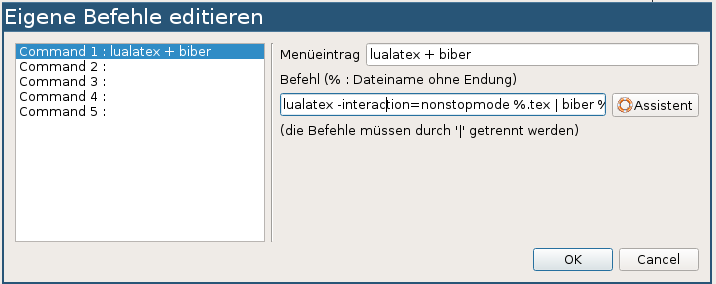
\includegraphics[width=12cm]{Plots/texmaker.png}
    \caption{Screenshot zur Erstellung des Kompilier-Befehls in Texmaker}
    \label{fig:texmaker}
\end{figure}


In Abbildung \ref{fig:texmaker} ist ein Screenshot des Befehlsmenü gezeigt. Ihren Befehl können Sie nun im Drop-Down-Menü zum 
Kompilieren des Dokuments auswählen und mit einem Klick auf den Pfeil starten.

\subsection{Aufräumen}

Nach einem \LaTeX-Fehler ist es oft notwendig, die erstellten Hilfsdateien zu löschen.
Klicken Sie hierzu auf \emph{Werkzeuge}→\emph{Aufräumen}.


\chapter{\LaTeX-Grundlagen}

Bitte beachten Sie beim Schreiben der Arbeit folgende Konventionen bzw. Grundlagen:

\begin{itemize}
    \item \textbf{Abschnitte und Zeilenumbrüche} \\
        Es sollten im Fließtext keine Zeilenumbrüche mit \textbackslash\textbackslash \ erzwungen werden.
        Schreiben Sie höchsten einen Satz in eine Code-Zeile.
        Absätze werden im Code mit einer Leerzeile markiert und dann entsprechend der Einstellung von \texttt{parskip} in der Dokumentenklasse gesetzt.
    \item \textbf{Kursiv/Aufrecht} \\
        \begin{itemize}
            \item Variablen und physikalische Größen werden kursiv gesetzt. 
            \item Einheiten werden immer aufrecht und mit einem halben Leerzeichen Abstand zur Zahl gesetzt. Nutzen Sie \texttt{siunitx}!
            \item Mathematische Konstanten und Funktionen werden ebenfalls aufrecht gesetzt. Zum Beispiel die Eulersche Zahl e, das imaginäre i und das infinitesimale d.
                Im Mathematikmodus können Sie dies mit dem Befehl \verb_\mathrm{}_ erreichen. Für die Funktionen stellt \LaTeX \ Befehle bereit, z.B. \verb+\arccos+.
            \item Integrand und ein $\mathrm{d}x$ sollten ebenfalls durch ein kleines Leerzeichen (\verb+\,+) getrennt werden.
        \end{itemize}
        


\end{itemize}

\section{Zahlen und Einheiten}

Jede Zahl, jede Einheit und jede Zahl mit Einheit sollte mit Hilfe der in dem Paket \texttt{siunitx} zur Verfügung gestellten Befehle gesetzt werden.
Grundsätzlich gilt: Einheiten werden aufrecht gesetzt und haben ein kleines Leerzeichen (\verb+\,+) Abstand zu ihrer Zahl. 
Werden Fließkommazahlen ohne \texttt{siunitx} gesetzt, entsteht ein hässlicher Leerraum zwischen Komma und erster Nachkommastelle, da \LaTeX \ das Komma nicht als Dezimaltrennzeichen, sondern als Satzzeichen interpretiert.

Das Paket wurde mit deutschen Spracheinstellungen (also mit Komma als Dezimaltrennzeichen und $\cdot$ zwischen Zahl und Zehnerpotenz) geladen, sowie mit den Einstellungen, dass die Standardabweichung stets durch $\pm$ abgetrennt wird und Einheiten falls nötig als Brüche ausgegeben werden.

\begin{table}
    \centering
    \caption{Beispiele für siunitx}
    \label{tab:si}
    \begin{tabular}{l r}
        \toprule
        Befehl     &   Ergebnis \\
        \midrule
        \verb+\num{1.2345}+ & \num{1.2345} \\
        \verb+\num{1.2e3}+ & \num{1.2e3} \\
        \verb_\num{1.2 +- 0.2}_ & \num{1.2+-0.2} \\
        \verb+\num{10000}+ & \num{10000} \\
        \verb+\si{\meter\per\second}+ & \si{\meter\per\second} \\
        \verb+\SI{1.2(1)}{\micro\ampere}+ & \SI{1.2(1)}{\micro\ampere} \\
        \verb+\SI{1.2\pm0.1e3}{\kilo\gram\per\cubic\meter}+ & \SI{1.2\pm0.1e3}{\kilo\gram\per\cubic\meter} \\
        \bottomrule 
    \end{tabular}
\end{table}

Das Paket stellt unter anderem die drei wichtigen Befehle
\begin{itemize}
    \item \texttt{\textbackslash num\{Zahl\}},
    \item \texttt{\textbackslash si\{Einheit\}} und
    \item \texttt{\textbackslash SI\{Zahl\}\{Einheit\}}
\end{itemize}
zur Verfügung.
Diese Befehle sollten stets genutzt werden, wenn Zahlen angegeben werden. 
Sie funktionieren sowohl im Text- als auch im Mathematikmodus.
In Tabelle \ref{tab:si} sind einige Beispiele aufgetragen. Bitte lesen Sie die Dokumentation \cite{siunitx}.

\section{Das Literaturverzeichnis}

Das Literaturverzeichnis wird mit Hilfe von BibLaTeX und biber erstellt.
Tragen Sie alle ihre Quellen in die Datei \texttt{references.bib} ein, Sie enthält bereits
einige Beispiele. Für weitere Informationen lesen Sie bitte die Dokumentation \cite{biblatex}.

Im Text können Sie mit \verb_\cite{kürzel}_ zitieren. Seitenzahlen geben Sie in eckigen Klammern an:
\verb_\cite[10]{kürzel}_. 

Das Literaturverzeichnis ist so eingestellt, dass es Ihre Quellen in alphabetischer Reihenfolge nach Autoren nummeriert.
Möchten Sie das Literaturverzeichnis nach der Reihenfolge des Auftauchens im Text sortieren, fügen sie die Paktetoption \texttt{sorting=none} beim Laden
des BibLaTeX-Pakets hinzu.

Den Zitier- und Bibliographie-Stil geben sie mit der Option \texttt{style=Stil} an. Die beiden gebräuchlisten Stile sind \texttt{numeric} und \texttt{alphabetic}. 
Bei \texttt{numeric} werden die Quellen durchnummeriert, bei \texttt{alphabetic} wird ein Buchstabenkürzel aus Autor(en)-Name(n) und Jahr verwendet.
Für weitere Stile konsultieren Sie bitte die Dokumentation: \cite{biblatex}.

Ein Beispiel für das Zitieren eines Buches lautet so \cite{handbook_adhesives},
wissenschaftliche Artikel hingegen werden so \cite{einstein} zitiert.

Damit das Literaturverzeichnis erstellt wird, ist ein Aufruf von \texttt{biber} nach einem ersten kompilieren mit \texttt{lualatex} nötig.
Danach muss das Dokument erneut mit \texttt{lualatex} kompiliert werden. 

Zum korrekten Kompilieren des Dokuments siehe Kapitel \ref{make}.

\chapter{Abbildungen und Tabellen}

\section{Abbildungen}

Achten Sie bei ihren Plots auf ausreichend große Achsenbschriftungen, ausreichende Schriftdicken und gut unterscheidbare Farben.
Im Idealfall haben Sie im Plot und der Arbeit die gleiche Schriftgröße und Schriftart.
Dies lässt sich durch Erstellen des Plots in der korrekten Größe und einbinden mit dem optionalen Argument \texttt{scale=1} erreichen. Ein Beispiel sehen Sie in Abbildung \ref{fig:bsp}.

Nutzen Sie wenn möglich Vektorgrafiken (pdf) und nur in Ausnahmen Rastergrafiken wie .png oder .jpg.
Setzen Sie Punkte hinter Abbildungsunterschriften.

\begin{figure}
    \centering
    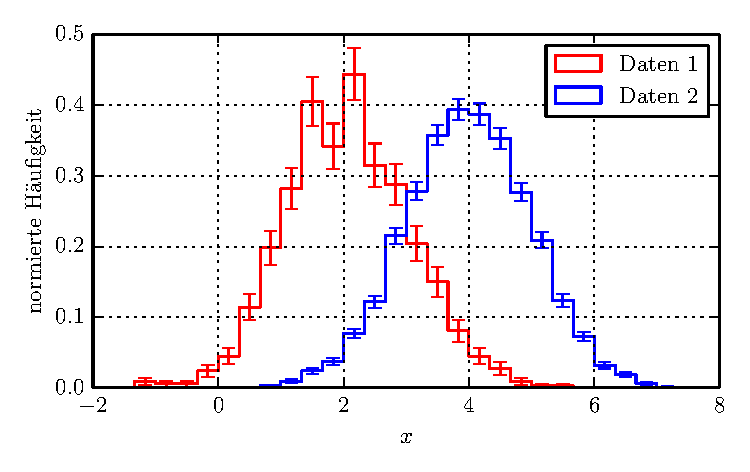
\includegraphics[scale=1]{./Plots/Histogramm.pdf}
    \caption{Ein Histogramm mit Fehlerbalken für zwei Datensätze, Schriftgröße und -art entsprechen der des Dokuments.}
    \label{fig:bsp}
\end{figure}

\section{Tabellen}

Tabellen sollten so einfach wie möglich aufgebaut sein, verzichten Sie auf zu viele Linien. In fast allen Fällen reichen drei horizontale Linien aus, jeweils über und unter der Tabelle und zwischen den Spaltenüberschriften und der eigentlichen Tabelle.

Das Paket \texttt{booktabs} stellt hierfür \verb_\toprule_, \verb_\midrule_ und 
\verb_\bottomrule_ zur Verfügung.
Das Paket \texttt{siunitx} stellt eine extrem mächtige neue Spalteneinstellung bereit: \texttt{S}, mit ihr können Zahlen und Einheiten sehr sauber und gut ausgerichtet gesetzt werden.

Diese Vorlage geht von Tabellenüberschriften aus, möchten Sie dagegen Tabellenunterschriften entfernen Sie das entsprechende optionale Argument für die Dokumentenklasse in der Präambel.

Ein Beispiel ist Tabelle~\ref{tab:bsp}.
\begin{table}
    \centering
    \caption{Beispieltabelle mit willkürlichen Werten, für die Zahlenwerte wurde die S-Option aus \texttt{siunitx} verwendet}
    \label{tab:bsp}
    \begin{tabular}{S[table-format=4.2] S[table-format=3.2]}
        \toprule
        {$p \mathrel{/} \si{\pascal}$}  & {$T \mathrel{/} \si{\kelvin}$} \\
        \midrule
        1024,23 & 273,15 \\
        1025,31 & 274,5 \\
        1026,27 & 276,2 \\
        \bottomrule
    \end{tabular}
\end{table}


\appendix
% Hier beginnt der Anhang, nummeriert in lateinischen Buchstaben
\chapter{Ein Anhangskapitel}

Hier könnte ein Anhang stehen, falls Sie z.B. Code, Konstruktionszeichnungen oder Ähnliches mit in die Arbeit bringen wollen. Im Normalfall stehen jedoch alle Ihre Resultate im Hauptteil der Bachelorarbeit und ein Anhang ist überflüssig.


\backmatter
\printbibliography

\cleardoublepage
\thispagestyle{empty}
\section*{Eidesstattliche Versicherung}
Ich versichere hiermit an Eides statt, dass ich die vorliegende Abschlussarbeit mit dem Titel \enquote{\thetitle} selbstständig und ohne unzulässige fremde Hilfe erbracht habe.
Ich habe keine anderen als die angegebenen Quellen und Hilfsmittel benutzt, sowie wörtliche und sinngemäße Zitate kenntlich gemacht. 
Die Arbeit hat in gleicher oder ähnlicher Form noch keiner Prüfungsbehörde vorgelegen.

\vspace*{1cm}\noindent
\begin{center}
  \begin{tabular}{@{}p{0.4\textwidth}@{\hspace{0.15\textwidth}}p{0.4\textwidth}@{}}
  \rule{\linewidth}{0.25pt}& \rule{\linewidth}{0.25pt}\\
  Ort, Datum & Unterschrift
  \end{tabular}
\end{center}

\subsection*{Belehrung}
Wer vorsätzlich gegen eine die Täuschung über Prüfungsleistungen betreffende Regelung einer Hochschulprüfungsordnung verstößt, handelt ordnungswidrig.
Die Ordnungswidrigkeit kann mit einer Geldbuße von bis zu \SI[round-mode=places, round-precision=2]{50000}{€} geahndet werden. 
Zuständige Verwaltungsbehörde für die Verfolgung und Ahndung von Ordnungswidrigkeiten ist der Kanzler/die Kanzlerin der Technischen Universität Dortmund. 
Im Falle eines mehrfachen oder sonstigen schwerwiegenden Täuschungsversuches kann der Prüfling zudem exmatrikuliert werden \mbox{(\S\,63 Abs. 5 Hochschulgesetz --HG--).}

Die Abgabe einer falschen Versicherung an Eides statt wird mit Freiheitsstrafe bis zu 3 Jahren oder mit Geldstrafe bestraft.

Die Technische Universität Dortmund wird ggf.\ elektronische Vergleichswerkzeuge (wie z.\,B.\ die Software \enquote{turnitin}) zur Überprüfung von Ordnungswidrigkeiten in Prüfungsverfahren nutzen. \\[\baselineskip]

\noindent Die oben stehende Belehrung habe ich zur Kenntnis genommen.\\[1cm]
\begin{center}
\begin{tabular}{@{}p{0.4\textwidth}@{\hspace{0.15\textwidth}}p{0.4\textwidth}@{}}
\rule{\linewidth}{0.25pt}& \rule{\linewidth}{0.25pt}\\
Ort, Datum & Unterschrift
\end{tabular}
\end{center}

\end{document}
